\section{Task 4 - Summary and Conclusions}

It's important to know that each floating point calculation if corrupted by
error so before analyzing the results it may be necessary to analyze if the
result is within satisfiable range of our precision. There is more to error of
the computation than just simple inaccuracy of value stored. Instead, each
calculation introduces more error.

\begin{figure}[ht]
    \begin{center}
        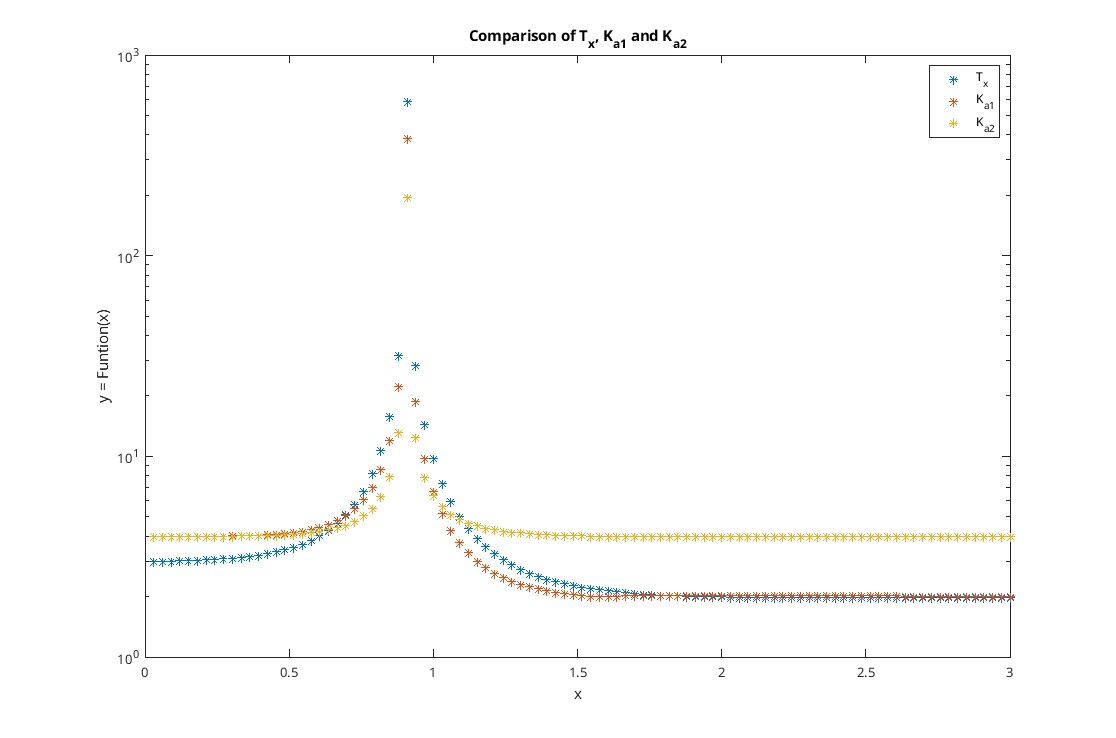
\includegraphics[width=\textwidth]{Task4.jpg}
    \end{center}
    \caption{Comparison of error from all 3 methods applied}
    \label{fig:task4}
\end{figure}

Different ways of calculating the same function can often have big impact on
the quality of the results. As one can clearly see from Figure \ref{fig:task4}
different methods yield different error results for the same input. In
particular, the difference between the $K_{a1}$ and $K_{a2}$, for $x\geq 1$ is
worthy of your attention. Furthermore, error introduced by the inaccurate
representation is different from the one that is introduced by the inaccurate
intermediate representation. Knowing that allows to design better, more
accurate algorithms. While developing and testing those methods it is ok to use
simplified formulas for calculating the error as they provide the same results
as the ones tailored to the specific problem.
